
\section{Test} % (fold)
\label{sec:test}
    
    I test sono stati condotti utilizzando le seguenti meta--euristiche.
    \begin{itemize}
        \item[--] \emph{simulated annealing} con mossa 3--modale SEO (\emph{Singleton} move, \emph{Even Chessboard} Move, \emph{Odd Chessboard} Move);
        \item[--] \emph{simulated annealing} con mossa 3--modale STL (\emph{Singleton} move, \emph{Three-Tile Streak} Move, \emph{L} Move);
        \item[--] \emph{steepest descent} con mossa 5--modale (\emph{Singleton} move, \emph{Even Chessboard} Move, \emph{Odd Chessboard} Move, \emph{Three-Tile Streak} Move, \emph{L} Move );
    \end{itemize}

    Sulla base delle funzioni offerte da easylocal++, la strategia \emph{steepest descent} con la mossa 5--modale chiama la BestMove usando l'enumerazione completa per le cinque mosse componenti. Per questo motivo, si è scelto di implementare la \emph{steepest descent} esternamente al framework, usando il \emph{tester} di easylocal++. In questo senso, si chiama il tester da terminale e si redirige in input a tale processo un file con i comandi per il tester, in modo che questi chiamino la BestMove delle cinque mosse. Un esempio è il seguente:

    \begin{lstlisting}
	 ./Eternity2 --main::instance "../eternity2-data/
	 pieces_set_2/e2pieces.txt" --main::seed 987 
	 < ../eternity2-data/ourInput/input_e2.txt | tail -n 50
	\end{lstlisting}

	I risultati verranno visualizzati tramite il seguente comando:

	\begin{lstlisting}
	java -jar e2visualizer.jar pieces_set_2/e2pieces.txt
	 ourSolutions/sol_e2.txt 1
	\end{lstlisting}
	




	\subsection{Simulated Annealing con mossa 3--modale SEO}
	L'istanza 03x03 è l'unica in cui siamo riusciti ad ottenere l'ottimo tramite simulated annealing.

	./Eternity2 --main::instance ../eternity2-data/pieces\_set\_2/pieces\_03x03.txt --main::seed 0 --main::method SEO\_SA --SEO\_SA::start\_temperature 10000 --SEO\_SA::min\_temperature 1 --SEO\_SA::cooling\_rate 0.99 --SEO\_SA::neighbors\_sampled 1000 --SEO\_SA::neighbors\_accepted 1000 --main::p1 0.70  --main::p2 0.15  --main::p3 0.15
	
	\begin{figure}[H]
	\centering
	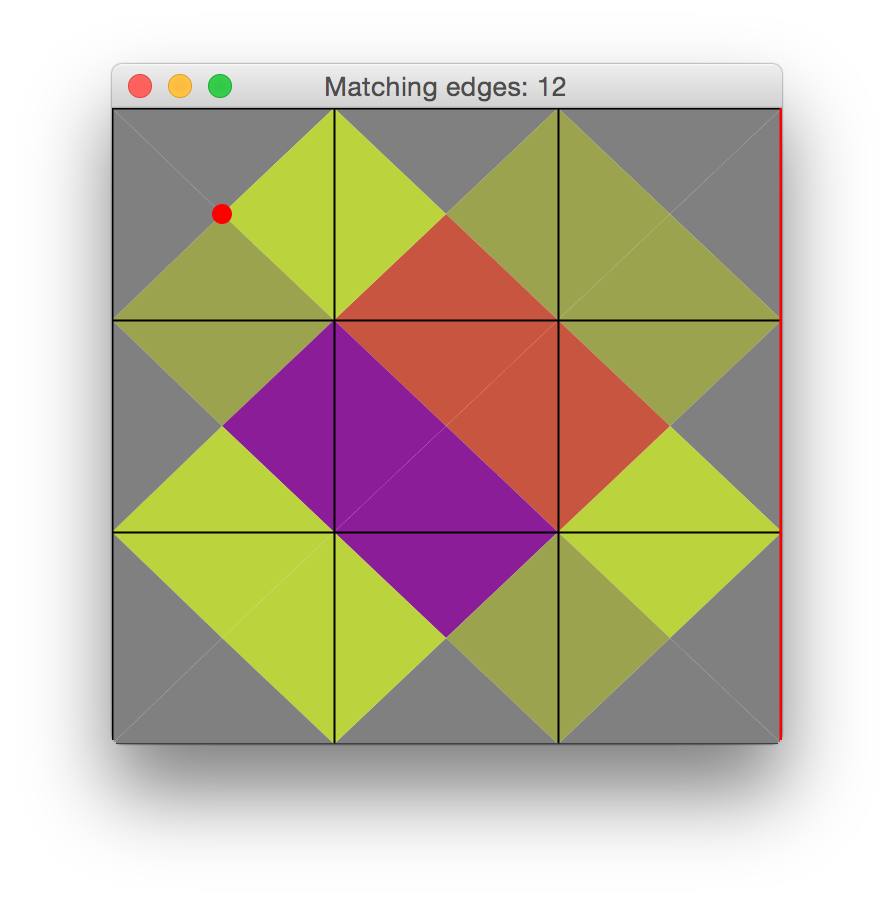
\includegraphics[scale=0.25]{img/sol_03x03_SA}
	\caption{Solution of the 3x3 board.}
	\end{figure}





	\subsection{Steepest Descent con mossa 5--modale}
	Come detto prima, si sono usati dei file interni per guidare il tester di easylocal++ durante la steepest descent. Questi file si trovano della cartella \emph{ourInput}. Nel seguito indicheremo i migliori risultati ottenuti tramite questa tecnica e la mossa 5--modale.

	\paragraph{03x03}
	./Eternity2 --main::instance ../eternity2-data/pieces\_set\_2/pieces\_03x03.txt --main::seed 24 $<$ ../eternity2-data/ourInput/input\_03x03.txt | tail -n 100

	\begin{itemize}
		\item COST = 0
		\item TIME = 0.027 sec
	\end{itemize}
	\begin{figure}[H]
	\centering
	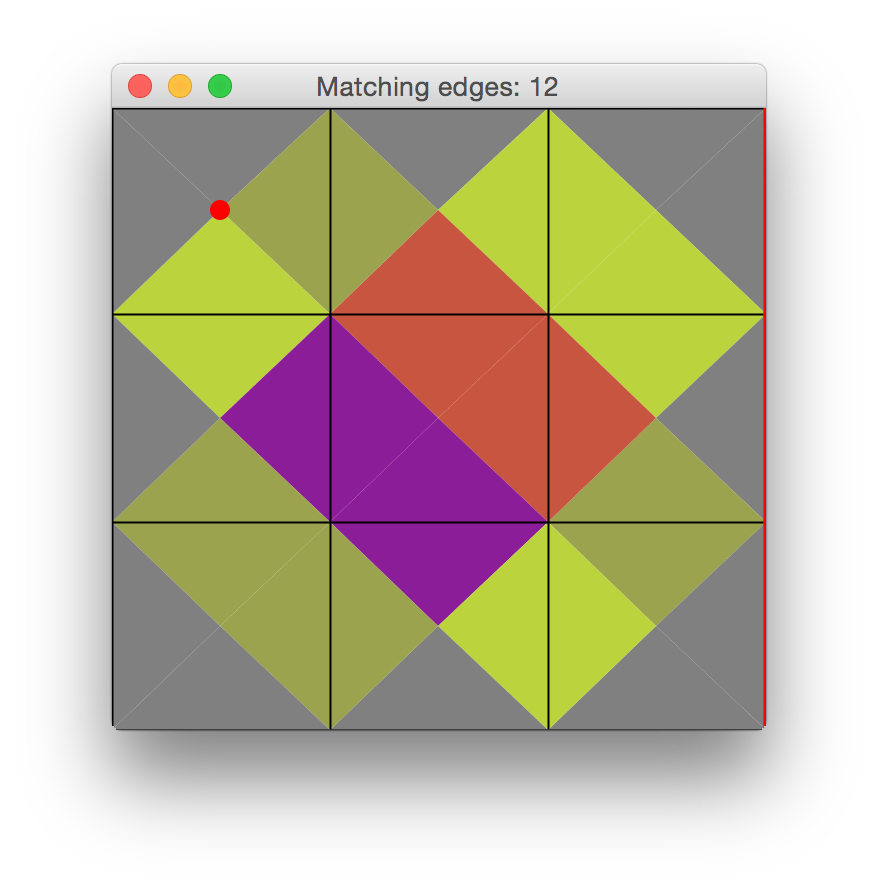
\includegraphics[scale=0.25]{img/sol_03x03}
	\caption{Solution of the 3x3 board.}
	\end{figure}



	\paragraph{04x04}
	./Eternity2 --main::instance ../eternity2-data/pieces\_set\_2/pieces\_04x04.txt --main::seed 26 $<$ ../eternity2-data/ourInput/input\_04x04.txt | tail -n 100

	\begin{itemize}
		\item COST = 0
		\item TIME = 0.057 sec
	\end{itemize}
	\begin{figure}[H]
	\centering
	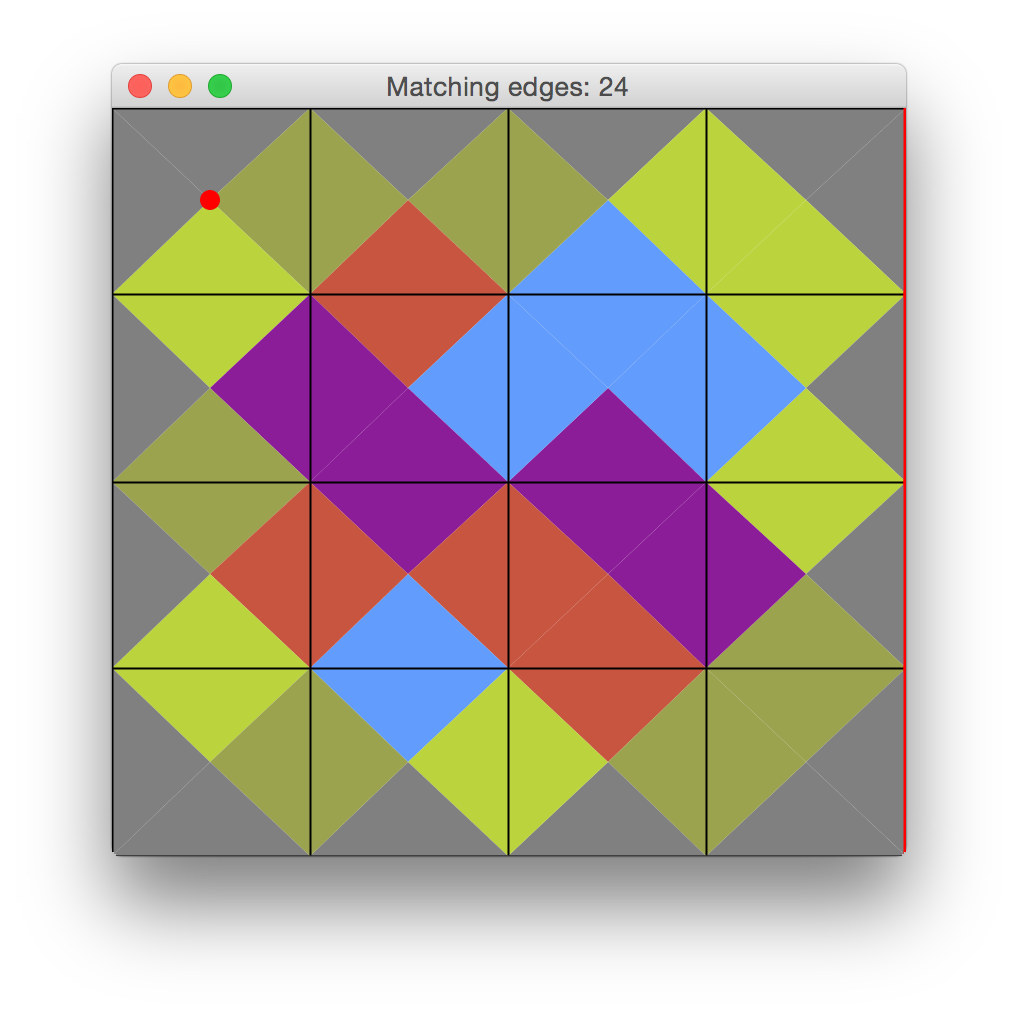
\includegraphics[scale=0.25]{img/sol_04x04}
	\caption{Solution of the 4x4 board.}
	\end{figure}



	\paragraph{05x05}
	./Eternity2 --main::instance ../eternity2-data/pieces\_set\_2/pieces\_05x05.txt --main::seed 987 $<$ ../eternity2-data/ourInput/input\_05x05.txt | tail -n 100

	\begin{itemize}
		\item COST = 2000
		\item TIME = 1.734 sec
	\end{itemize}
	\begin{figure}[H]
	\centering
	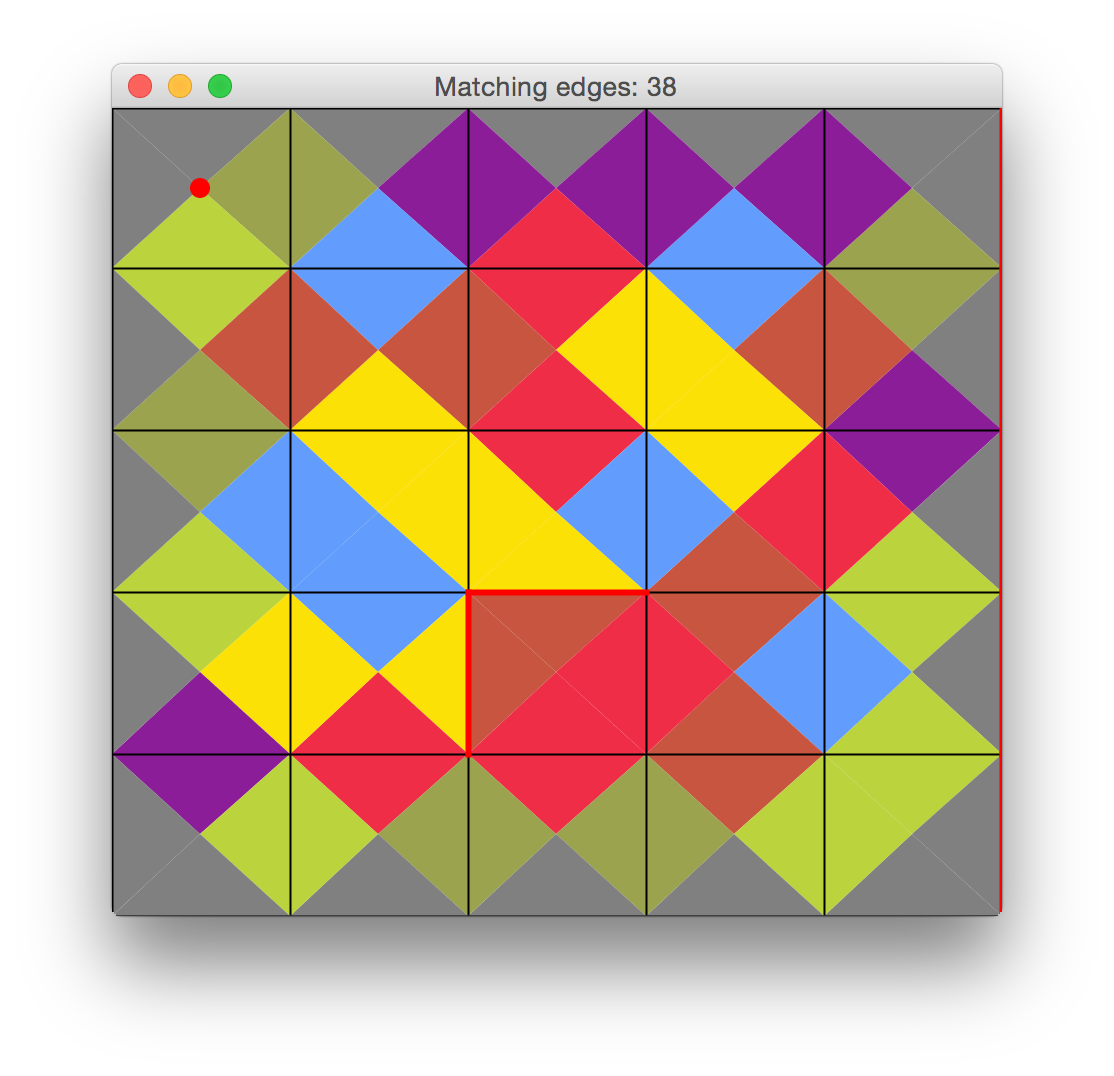
\includegraphics[scale=0.25]{img/sol_05x05}
	\caption{Solution of the 5x5 board.}
	\end{figure}


	\paragraph{Eternity 2 originale}
	./Eternity2 --main::instance ../eternity2-data/pieces\_set\_2/e2pieces.txt --main::seed 987 $<$ ../eternity2-data/ourInput/input\_e2.txt | tail -n 100

	\begin{itemize}
		\item COST = 62000
		\item TIME = 3 m 40 sec
	\end{itemize}
	\begin{figure}[H]
	\centering
	\includegraphics[scale=0.5]{img/sol_e2}
	\caption{Solution of Eternity 2.}
	\end{figure}














% section test (end)